\section{FIT Allokáció} \label{sec:fit_allocation}
Az ipari rendszerek egyre összetettebbekké váltak az évek során. 
Emellett mostanság egyre több ilyen rendszer tartalmaz elektronikát és szoftvert, 
tehát a funkcionális biztonságnak folyamatosan nő a fontossága. (Schabe, 2018 \cite{Schabe})

A safety integrity level (SIL) egy diszkrét érték ami meghatározza a használandó módszereket, technikákat a véletlenszerű és szisztematikus hibák elkerülése érdekében.
A SIL-ek koncepciója már több szabvány rendszerben ki lett fejlesztve.
Ezek között legismertebb szabványok az IEC 61508, DEF-STAN-0056, EN 50126, EN 50128, EN 50129 és még sok más.

A SIL-nek két fő aspektusa van:
\begin{enumerate}
    \item Egy cél hibaráta, amit a rendszernek nem szabad meghaladni, hogy tudja kezelni a véletlen hibákat
    \item Módszerek és technikák halmaza, amit a szisztematikus hibákat kezeli 
\end{enumerate}

Itt fontos megjegyezni, hogy szoftverben csak és kizárólag szisztematikus hibákat vesznek figyelembe és nincs megadva cél hibaráta. Ez abból adódik, hogy a szoftverben nincs véletlenszerű hiba.

\subsection{Különböző SIL-ek}
A \ref{tab:SILs} táblázat példát ad a SIL-ek és a tűrhető hibaráta kapcsolatára, ahogy három szabvány, az IEC 61508, az EN 50129 és a DEF-STAN-0056 definiálja.

A tűrhető hibaráta (THR) egy eszköz veszélyes hibáinak maximális rátája, amit a szabvány definiál bizonyos safety integrity szinthez.
Látni kell azt, hogy bár az IEC és EN szabványoknál azonosak a THR értékek, a DEF-STAN-0056-ban eltér.
Ezért a szabványok közti átjárás nem mindig triviális.
Attól még, hogy a THR értékek hasonlóak az IEC és EN szabványok között, az rendszer szintű hibaelkerülő módszerek különböznek, ezért ezek a SIL-ek sem ugyan azok.
\begin{table}[ht]
	\footnotesize
	\centering
	\begin{tabular}{ l c c }
		\toprule
		SIL & IEC 61508/EN 50129 & DEF-STAN-0056 \\
		\midrule
		1 & \(10^{-6}/h \leq\) THR \(< 10^{-5}/h\) & Frequent \(\approx 10^{-2}/h\)\\
		2 & \(10^{-7}/h \leq\) THR \(< 10^{-6}/h\)  & Probable \(\approx 10^{-4}/h\)\\
		3 & \(10^{-8}/h \leq\) THR \(< 10^{-7}/h\)  & Occasional \(\approx 10^{-6}/h\)\\
		4 & \(10^{-9}/h \leq\) THR \(< 10^{-8}/h\)  & Remote \(\approx 10^{-8}/h\) \\
		\bottomrule
	\end{tabular}
	\caption{SIL értékek több szabvány és THR szerint}
	\label{tab:SILs}
\end{table}

\subsection{Safety integrity szintek kombinációja}
Ebben a részben a különböző szabványok SIL szintjeinek kombinációját mutatom be.

\subsubsection{DEF-STAN-0056}
A szabvány a következő szabályokat definiálja a 7.4.4. rész 5.8. táblázatában:
\begin{itemize}
	\item Két SIL3 eszköz párhuzamos kombinációjaként létrejövő rendszer SIL4-es besorolású lesz.
	\item Két SIL2 eszköz párhuzamos kombinációjaként létrejövő rendszer SIL3-es besorolású lesz.
	\item Két SIL1 eszköz párhuzamos kombinációjaként létrejövő rendszer SIL2-es besorolású lesz.
	\item Két eszköz párhuzamos kombinációjaként - ahol az eszközök rendre SIL X és SIL Y besorolásúak - létrejövő rendszer SIL értéke SIL max(x,y).
\end{itemize}

Az olvasót a szabvány figyelmezteti, hogy ne keverje össze ezeket a szabályokat az EN 20129\cite{EN50129} által definiált safety integrity szintekkel.

Továbbá jelen esetben a "párhuzamos kombináció" azt jelenti, hogy a két eszköz vagy funkció úgy van társítva, hogy a veszélyes hiba kiváltásához mind a két eszköz hibája szükséges.

\subsubsection{IEC 61508}
A szabvány nem rendelkezik előre definiált szabályokkal, mint a fenti esetben, de ad némi lehetőséget magasabb integritási szint elérésére kombinációk által.
Az általános szabály a következő (lásd IEC 61508-2, 7.4.4.2.4. rész):
\begin{center}
	Selecting the channel with the highest safety integrity level that has been achieved for the safety funciton under consideration and the adding N safety integrity levels to determing the maximum safety integrity level for the overall combination of the subsystem.
\end{center}

Itt N a párhuzamos kombinációban résztvevő elemek hardverhiba tűrése, azaz hány veszélyes hibát tud a rendszer tolerálni.
Továbbá a rendszerek/elemek között is létezik megkülönböztetés, A és B típus. 

Egy elem A típusúnak mondható, ha a biztonsági funkció eléréséhez a következők teljesülnek:
\begin{enumerate}
	\item A komponens alkotórészeinek összes hibamódja jól körülhatárolt.
	\item Hiba esetén a komponens viselkedése teljes mértékben meghatározható.
	\item Létezik elegendő megbízható meghibásodási adat, ami bizonyítja az állított hibarátát.
\end{enumerate}
Minden más elem/rendszer a B kategóriába kerül.

A követelményeknek való megfelelésből is látszik, hogy a szabvány nem ad egyszerű szabályokat a integritási szintek elosztásáról. 
Nem csak a rendszerek elrendezése és ez által a hardveres hibatűrése határozza meg a SIL-t, hanem még a rendszer biztonsági hiba hányada (Safe Failure Fraction [SSF]) is.
Az SSF meghatározásának módját a szabvány C függelékében definiálja.

\subsubsection{SIRF 400}
A Sicherheitsrichtlinie Farhrzeug (SIRF) a németországi rendelet a vasúti járművek biztonságára. 
Németországban könnyű hivatkozni erre a dokumentumra, de az ország határain kívül nem biztosított az autómatikus megfelelése.

A dokumentum SIL allokáció problémájára a következő elveket adja.

Két alrandszer soros összeköttetése (például: hibafában VAGY kapuval összekötve) esetén, a legkisebb SIL érték határozza meg az összekapcsolt rendszer integritási szintjét.

A párhuzamos kombinációkhoz a következő szabályok adottak:
\begin{enumerate}
	\item Egy SIL > 0 rendszer nem állítható össze SIL 0 elemekből.
	\item Egy integritási szint elengedhető maximum egy szinttel egy ÉS kapu alatt.
	\item Kizárás a 2. pont alól: Egy ág teljesen átveszi a biztonsági funkciót.
	\item Kizárás a 2. pont alól: Common cause failure analízis kivitelezésre került.
	\item A 4. pont esetében egy megfelelő szisztematikus módszert (FMEA, HAZOP, etc.) a hibafa legalsóbb szintjéig kell alkalmazni, hogy bebizonyosodjon a CCF kizárásának lehetősége.
\end{enumerate}
Az \ref{fig:sirfSIL}. ábrán látható a SIRF által megengedett kombinációk. 
Az ábrákon zöld szín jelzi a megengedett, prios szín a tiltott kombinációkat és a fehér jelöli azokat, amikhez további elemzést kell végrehajtani, ami megmutatja az alegységek függetlenségét.

\begin{figure}[!ht]
	\centering
	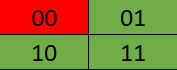
\includegraphics[width=67mm, keepaspectratio]{figures/sirf_sil1.png}\hspace{1cm}
	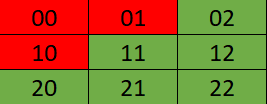
\includegraphics[width=67mm, keepaspectratio]{figures/sirf_sil2.png}\\\vspace{1cm}
	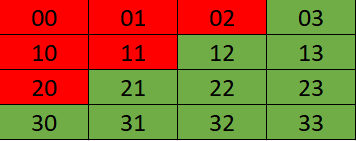
\includegraphics[width=67mm, keepaspectratio]{figures/sirf_sil3.png}\hspace{1cm}
	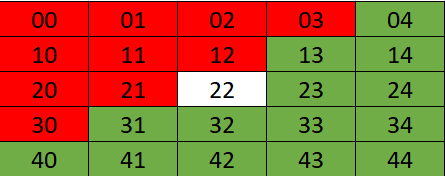
\includegraphics[width=67mm, keepaspectratio]{figures/sirf_sil4.png}
	\caption{Megengedett kombinációk az integritás szinteknek megfelelően \emph{Forrás}: SIRF 400}
	\label{fig:sirfSIL}
\end{figure}

\subsubsection{EN 50129}
Hazard to last independent function.
Ezután TFFR és SIL Allocation.
A funkciók alrészeinél a TFFR további bontása, de megmarad a SIL, performed by a suitable representation of the combination logic (RBD, FTA, Binary Decision D, Markov, Petri, etc).

SIL allocation, functions controlling the same hazard, SILs shall be allocated according to the TFFR.
For a function controlling multiple hazards, if derivation of TFFR apportionment and SIL allocation are preformed separately for each hazard, most restrictive shall apply.